\section{Investment}\label{subsec: distance investment}
In this section, we consider the investment setting. Notice that the incentive of the agent is the same as before. The main difference between this setting and the manipulation setting is the incentive of the principal. All omitted proofs in this section are provided in \cref{appendix: distance investment}.
% We show that the optimal mechanism is a simultaneous mechanism when the agent invests (\cref{thm:distance cost investment optimal mech}).

\subsection{Optimal sequential mechanism}
First, we  show that under a mild condition, there exists a random-order mechanism without disclosure that can achieve the first best (\cref{thm: true effort sequential}).



\begin{theorem}\label{thm: true effort sequential}
% Consider  the investment setting. 
    % Suppose the cost is induced by the Euclidean distance and is additive.
    If $\theta\geq 30^{\circ}$, for any distribution $\dist$, 
   then the   random order mechanism without disclosure $(\classifier_A,\classifier_B,\frac12,\nullset)$ achieves the first best.
\end{theorem}

\begin{lemma}\label{claim same behavior}
    If $\theta\geq 30^{\circ}$, then in $(\classifier_A,\classifier_B,\frac12,\nullset)$, any attributes $\features\notin \classifier_A\cap\classifier_B$ that get accepted by this mechanism use a one-step strategy.
\end{lemma}



\begin{proof}[Proof of \cref{thm: true effort sequential}]
   By \cref{claim same behavior}, any agent that gets selected adopt some attributes in $\classifier_A\cap\classifier_B$ under the random-order mechanism $(\classifier_A,\classifier_B,\frac12,\nullset)$.
    We show that the described mechanism selects all potential qualified agents and zero unqualified agent, which achieves the first best.
   First, any qualified agent gets selected with zero cost under the described mechanism.
    Second, notice that under the investment setting, every unqualified agent who can improve to some qualified attributes with cost less than one become qualified.
    Such an agent is selected by the described mechanism.
    % Consider an unqualified agent with attributes $\features\not\in\classifier_A \cap \classifier_B$. 
    % Suppose there exists attributes $\features'$ such that (1)  $\features'$ satisfy both tests $\classifier_A$ and $\classifier_B$; and (2)  such an agent can move to $\features'$ with cost $c(\features, \features', \features') \leq 1$.
    % Then this unqualified agent has an incentive  to improve his attributes to $\features'$ and get accepted.  
    % However, if instead such attributes $\features'$ do not exist and for any attributes $\features''$ in $\classifier_A \cap \classifier_B$, the cost for this agent with attributes $\features$ to improve to $\features''$ is strictly larger than one, then this unqualified agent has no incentive to move to the qualified region $\classifier_A \cap \classifier_B$ in any mechanism.
    Third, any other attributes can only get selected by the described mechanism with a cost strictly larger than one, which is profitable.
    So these attributes remain unqualified and are not selected.
\end{proof}

%--------------------------------------------
\cref{thm: true effort sequential} hinges that in  the investment setting, the key for any sequential mechanism to achieve the first best is that every agent prefers using some one-step strategy in the sequential mechanism.
This observation will be made concrete in \cref{lem: optimal max qualified improving effort}.

How do other sequential mechanisms perform when the agent invests?
First, if $\theta<90^{\circ}$, there does not exist any sequential mechanism with fixed order that can achieve the first best.
Consider the fixed-order sequential mechanism that first offers $\classifier_A$ and then $\classifier_B$.
Under this mechanism, some attributes prefer using a two-step strategy and they do not become qualified after the investment. 
For example, in \cref{subfig:BR sequential fixed},  the agent with attributes $\orifeatures$ (on the boundary line of $\classifier_A$) uses the following strategy: he does not change his attributes before the first test, and invests to become $\secondfeatures$ (its projection on the boundary line of $\classifier_B$) before the second test.
Although this agent passes both tests and gets selected under the current mechanism, he is still unqualified after investment.
To prevent selecting any unqualified agent, the principal needs to use at least one stringent test under this mechanism.
For example, offering $\tilde{\classifier}_A$ first and then $\classifier_B$ as shown in \cref{fig:feasible fixed improvement}. 
% By using test $\tilde{\classifier}_A$ which is more stringent than $\classifier_A$, even for those attributes who use a two-step strategy would improve to the qualified region. 

    \begin{figure}[t]
\centering
\begin{subfigure}[b]{0.45\linewidth}
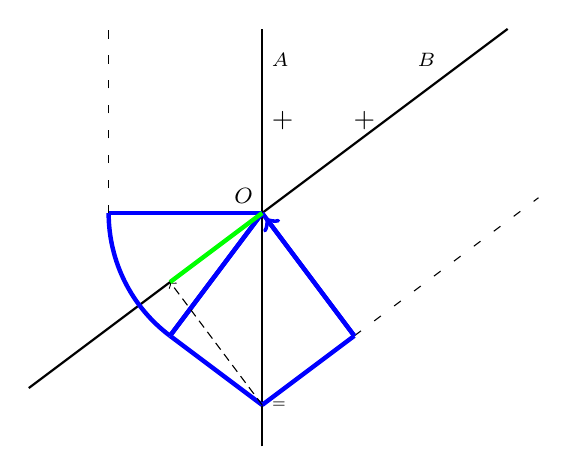
\begin{tikzpicture}[xscale=7.8,yscale=7.8]

\draw [domain=0.62:1.4, thick] plot (\x, {3/4*\x+1/4});
\node [left] at (1.3, 1.25 ) {$ \classifier_B$};%:\feature_2\geq \frac34 \feature_1 +\frac14
\draw [thick] (1,0.62) -- (1,1.3);
\node [right] at (1, 1.25) {$\classifier_A$};%: \feature_1 \geq 1$
\node [above,font=\tiny] at (0.97, 1 ) {\footnotesize$O$};
\node [left] at (1.2,1.15) {$+$};
\node [right] at (1, 1.15) {$+$};

\draw [domain=1+0.25*0.6:1.45, loosely dashed] plot (\x, {3/4*\x+1/4-5/16}); % 1/c = 1/4
% \node [below] at (1.6, 1.45-5/16 ) {$\classifier_2^-$}; %:\feature_2\geq \frac34 \feature_1 -\frac{1}{16}
\draw [loosely dashed] (1,1) -- (1+0.25*0.6,1-0.25*0.8);

\draw [loosely dashed] (1-0.25,1) -- (1-0.25,1.3);
% \node [right] at (1-0.25, 1.3 ) {$\classifier_1^-$};
\draw [loosely dashed] (1-0.25,1) -- (1,1);



\draw[blue, ultra thick] (1-0.25,1) arc (180:233.1:0.25);
\draw[blue, ultra thick] (1,1) -- ++(180:0.25);
\draw[blue, ultra thick] (1,1) -- ++(233.1:0.25) ;



\draw [blue, ultra thick] (1,1) -- (1-0.25*0.6,1-0.25*0.8);

\draw [ blue, ultra thick] (1,11/16) -- (1-0.25*0.6,1-0.25*0.8);

\draw [blue, ultra thick] (1,11/16) -- (1+0.25*0.6,1-0.25*0.8);
\draw [blue, ultra thick] (1,1) -- (1+0.25*0.6,1-0.25*0.8);
\draw [blue, ultra thick, <-] (1+0.01*0.6,1-0.01*0.8) -- (1+0.25*0.6,1-0.25*0.8);



\node [right, font=\tiny] at (1,11/16) {$\orifeatures=\firstfeatures$};

\draw [densely dashed, ->]  (1,11/16) -- (1-0.15, 1-0.15*3/4);
\draw [ultra thick, green]  (1,1) -- (1-0.15, 1-0.15*3/4);
\node [left, font=\tiny] at (1-0.15, 1-0.15*3/4) {$\secondfeatures$};

\end{tikzpicture}
\caption{BR in fixed order mech: $\classifier_A\rightarrow\classifier_B$ }
\label{subfig:BR sequential fixed}
\end{subfigure}
  \begin{subfigure}[b]{0.45\linewidth}
\begin{tikzpicture}[xscale=7.6,yscale=7.6]

\draw [domain=0.66:1.4, thick] plot (\x, {3/4*\x+1/4});
\node [left] at (1.36, 1.28 ) {$\classifier_B$};%:\feature_2\geq \frac34 \feature_1 +\frac14
\draw [thick] (1,0.66) -- (1,1.3);
\node [right] at (1, 1.28) {$\classifier_A$};%: \feature_1 \geq 1$
\node [above,font=\tiny] at (0.97, 1 ) {\footnotesize$O$};
% \node [left] at (1.2,1.15) {$+$};
% \node [right] at (1, 1.15) {$+$};


\draw [domain=1+0.25*0.6:1.45, densely dashed] plot (\x, {3/4*\x+1/4-5/16}); 
\draw [densely dashed] (1,1) -- (1+0.25*0.6,1-0.25*0.8);

\draw [densely dashed] (1-0.25,1) -- (1-0.25,1.3);
\draw [densely dashed] (1-0.25,1) -- (1,1);

\draw[densely dashed] (1-0.25,1) arc (180:233.1:0.25);
\draw[densely dashed] (1,1) -- ++(180:0.25);
\draw[densely dashed] (1,1) -- ++(233.1:0.25) ;


\draw [densely dashed] (1,1) -- (1-0.25*0.6,1-0.25*0.8);
\draw [ densely dashed] (1,11/16) -- (1-0.25*0.6,1-0.25*0.8);
\draw [densely dashed] (1,11/16) -- (1+0.25*0.6,1-0.25*0.8);
\draw [densely dashed] (1,1) -- (1+0.25*0.6,1-0.25*0.8);



\draw [ultra thick, red] (1+0.25*0.6,0.66) -- (1+0.25*0.6,1.3);


\draw [<->, red, dotted] (1,1.16) -- (1+0.25*0.6,1.16);
\node [above, red] at (1+0.07, 1.16 ) {$\frac{\cos{\theta}}{\eta}$};
\node [right,red] at (1+0.25*0.6, 1.28) {$\tilde\classifier_A$};%: \feature_1 \geq 1$
% \draw [domain=0.6:1.4, thick, teal] plot (\x, {3/4*\x+1/4});




\draw[blue, ultra thick] (0.9,3/4*1.15+1/4) arc (180:233.1:0.25);
\draw[blue, ultra  thick] (1.15,3/4*1.15+1/4) -- ++(180:0.25);
\draw[blue, ultra  thick] (1.15,3/4*1.15+1/4) -- ++(233.1:0.25) ;

\draw [blue, ultra  thick] (1.15,3/4*1.15+1/4-5/16) -- (1.15-0.25*0.6,3/4*1.15+1/4-0.25*0.8);

\draw [blue, ultra thick] (1.15,1.15*0.75+0.25) -- (1.15+0.25*0.6,3/4*1.15+1/4-0.25*0.8);

% \node [below, font=\tiny, red] at (1.2,3/4*1.15+1/4-5/16) {\footnotesize$C'$};
\draw [blue, ultra thick] (1.15,3/4*1.15+1/4-5/16) -- (1.15+0.25*0.6,3/4*1.15+1/4-0.25*0.8);

\draw [densely dashed]  (1,1) -- (1.15,3/4*1.15+1/4);
\draw [ultra thick, green]  (1,1) -- (1.15,3/4*1.15+1/4);



\end{tikzpicture}
\caption{Feasible mechanism: tests $\tilde\classifier_A,\classifier_B$} 
\label{fig:feasible fixed improvement}
  \end{subfigure}
\caption{One feasible sequential mechanism with fixed order}

\end{figure}

Moreover, a random-order mechanism that discloses the first test result to the agent is usually worse than some fixed order mechanism.
We formally prove this observation in \cref{prop:investment fixed order better than informed}.
% To provide intuition, consider the mechanism $(\classifier_A,\classifier_B,\frac12,\test_1)$as in \cref{subfig:ex random informed}.
% Consider the attributes $C$ that lie on the boundary line of $\classifier_A$ whose distance to the boundary line of $\classifier_B$ is $1/\eta$ (See \cref{subfig:ex random informed}).
% Notice that if the agent with attributes $C$ were to move to $\classifier_A\cap\classifier_B$, the cost exceeds one, which makes it not profitable for such an agent to use any one-step strategy.
% However, under the informed random order mechanism, the agent with attributes $C$ can wait in the first test; 
% if he is informed to have passed the first test, he could then move to $\classifier_B$ with a cost $1$ and get selected.
% Such a strategy makes this agent break-even and get selected with probability $1/2$.


% \begin{figure}
%     \centering
%       \begin{subfigure}[b]{0.45\linewidth}
% \begin{tikzpicture}[xscale=7.8,yscale=7.8]

% \draw [domain=0.66:1.4, thick] plot (\x, {3/4*\x+1/4});
% \node [left] at (1.3, 1.25 ) {$\classifier_B$};%:\feature_2\geq \frac34 \feature_1 +\frac14
% \draw [thick] (1,0.66) -- (1,1.3);
% \node [right] at (1, 1.25) {$\classifier_A$};%: \feature_1 \geq 1$
% \node [above,font=\tiny] at (0.97, 1 ) {\footnotesize$O$};
% \node [left] at (1.2,1.15) {$+$};
% \node [right] at (1, 1.15) {$+$};

% \draw [domain=1+0.25*0.6:1.45, loosely dashed] plot (\x, {3/4*\x+1/4-5/16}); % 1/c = 1/4
% \draw [dotted] (1,1) -- (1+0.25*0.6,1-0.25*0.8);

% \draw [loosely dashed] (1-0.25,1) -- (1-0.25,1.3);
% \draw [loosely dashed] (1-0.25,1) -- (1,1);


% \draw[blue] (1-0.25,1) arc (180:360-53.1:0.25);
% \draw[blue] (1,1) -- ++(180:0.25);
% \draw[blue] (1,1) -- ++(360-53.1:0.25) ;


% \end{tikzpicture}
% \caption{ $(\classifier_A,\classifier_B,0.5,\nullset)$} 
% \label{subfig:ex random uninformed}
% \end{subfigure}
% \begin{subfigure}[b]{0.45\linewidth}
% \centering
% \begin{tikzpicture}[xscale=7.8,yscale=7.8,
%     pics/legend entry/.style={code={%   
%         \draw[pic actions] 
%         (-0.25,0.25) -- (0.25,0.25);}}]

% \draw [domain=0.66:1.4, thick] plot (\x, {3/4*\x+1/4});
% \node [left] at (1.3, 1.25 ) {$\classifier_B$};%:\feature_2\geq \frac34 \feature_1 +\frac14
% \draw [thick] (1,0.66) -- (1,1.3);
% \node [right] at (1, 1.25) {$\classifier_A$};%: \feature_1 \geq 1$
% \node [above,font=\tiny] at (0.97, 1 ) {\footnotesize$O$};
% \node [left] at (1.2,1.15) {$+$};
% \node [right] at (1, 1.15) {$+$};


% \draw [domain=1+0.25*0.6:1.45, loosely dashed] plot (\x, {3/4*\x+1/4-5/16}); 
% \draw [loosely dashed] (1,1) -- (1+0.25*0.6,1-0.25*0.8);

% \draw [loosely dashed] (1-0.25,1) -- (1-0.25,1.3);
% \draw [loosely dashed] (1-0.25,1) -- (1,1);

% \draw [blue] (1-0.25,1) -- (1-0.25,{3/4*0.75+1/4});
% \node [left, font=\tiny] at (1-0.25, 1 ) {\footnotesize$A$};

% \node [left, font=\tiny] at (1-0.25, {3/4*0.75+1/4} ) {\footnotesize$B$};


% \draw[blue]  (0.93 ,{-1/sqrt(1/0.72^2-1)*(0.93-1)+11/16}) arc (254.1:232.8:0.25);

% \draw[blue] (1,1) -- ++(180:0.25);
% \draw[ blue] (1,1) -- ++(360-53.1:0.25) ;

% % \draw [teal, densely dashed] (1,1) -- (1-0.25*0.6,1-0.25*0.8);
% % \draw [domain=1-0.25*0.6:1, teal, densely dashed] plot (\x, {-3/4*(\x-1)+11/16}); 
% %\node [below] at (1-0.25*0.6,1-0.25*0.8) {\footnotesize$B'$};

% % \draw [ red, loosely dashed] (1,1) -- (1+0.25*0.6*0.9,1-0.25*0.8*0.9);

% % \draw [ red, ] (1,1) -- ({1-sqrt(1-0.72^2)*0.25*0.5},{1/sqrt(1/0.72^2-1)*sqrt(1-0.72^2)*0.25*0.5+11/16});


% % \node [below] at (1+0.25*0.6,1-0.25*0.8) {\footnotesize$B$};
% \draw [blue] (1,11/16) -- (0.94,{-1/sqrt(1/0.72^2-1)*(0.94-1)+11/16});
% \node [right] at (1,11/16) {\footnotesize$C$};
% \draw [blue] (1,11/16) -- (1+0.25*0.6,1-0.25*0.8);

% \draw [domain=0.93:1, blue] plot (\x, {-1/sqrt(1/0.72^2-1)*(\x-1)+11/16}); 
% % \node[below] at (0.93 ,{-1/sqrt(1/0.72^2-1)*(0.93-1)+11/16}) {\footnotesize$D$};

%  \draw [domain=1-0.25:0.85, blue] plot (\x, {tan(-7.075621914)*(\x-0.75)+13/16}); 


% % \matrix [draw, above right] at (1.3,0.7) {
% % \pic[blue]{legend entry}; &  \node[blue,font=\tiny] {$\setO$}; \\
% %  \pic[red]{legend entry}; &  \node[red,font=\tiny] {$\setonetwo_{0.5,\{\test_1\}}$}; \\
% %  \pic[teal, densely dashed]{legend entry}; &  \node[teal,font=\tiny] {$\setonetwo_{1,\nullset}$}; \\
% % };

% \end{tikzpicture}
% \caption{$(\classifier_A,\classifier_B,0.5,\{\test_1\})$} 
% \label{subfig:ex random informed}
%   \end{subfigure}
% \caption{Best response in random order mechanisms}  
%     \label{fig:random informed}
% %     \rule{0in}{1.2em}$^\dag$\scriptsize 
% % The set of candidates who get selected under the random order mechanism $(\classifier_A,\classifier_B,0.5,\{\test_1\})$ is \\
% \end{figure}

What happens when $\theta\leq 30^{\circ}$?
When $\theta< 30^{\circ}$, depending on the distribution, both random-order mechanisms without disclosure and fixed-order mechanisms could be optimal.
To provide intuition, consider the mechanism $(\classifier_A,\classifier_B,\frac12,\nullset)$ and $\theta<30^{\circ}$ as in  \cref{fig:theta<30 random}.
$\theta<30^{\circ}$ can be interpreted as the two requirements set by the principal are significantly in conflict with each other .
Hence there exists some attributes that  satisfy neither $\classifier_A$ and $\classifier_B$ would find it very costly to satisfy both tests simultaneously, but the small angle allows them to use a two-step strategy in the random-order mechanism without disclosure.
For example, $\orifeatures$ in  \cref{fig:theta<30 random}.
However, in the investment setting, when these attributes use a two-step strategy, their eventual attributes are still unqualified under non-stringent tests $\classifier_A$ and $\classifier_B$.

To make this mechanism feasible, two stringent tests are required.
For example, the two tests $\classifier_A^*$ and $\classifier_B^*$ shifted by a distance of $\frac{1}{2\eta}$ as in \cref{fig:theta<30 random}.
This incurs a loss: some unqualified attributes that could have improved to the qualified region would no longer be accepted under the feasible random-order mechanism without disclosure.
In contrast, as we have argued above, a feasible fixed-order mechanism only requires using one stringent test (See \cref{fig:feasible fixed improvement}).
After using stringent tests, the set of agent that will be accepted under a fixed-order mechanism and that under a random-order mechanism without disclosure no longer have a nested structure.
Hence depending on the distribution, either could be better.



       \begin{figure}[t]
\centering
\begin{tikzpicture}[xscale=4.3,yscale=4.3,
    pics/legend entry/.style={code={%   
        \draw[pic actions] 
        (-0.25,0.25) -- (0.25,0.25);}}]]

\draw [domain=0.85:1.26, thick] plot (\x, {tan(deg(0.4*pi))*(\x-1)+1});%less than pi/9
% \node [right] at (1.12, 1.34) {$\classifier_B$};
% \node [left] at (1, 1.34 ) {$\classifier_A$};
\draw [thick] (1,0.54) -- (1,1.8);


\draw [domain={1+0.25*cos(deg(0.1*pi))}:1.5, loosely dashed] plot (\x, {tan(deg(0.4*pi))*(\x-1)+1-0.809}); % 1/c = 1/4
\draw [loosely dashed] (1-0.25,1) -- (1-0.25,1.76);
\draw[red, ultra thick] (1-0.25,1) arc (180:240:0.25);
\draw[red, ultra thick] (1,1) -- ++(180:0.25);
% \draw[red] (1,1) -- ++(240:0.25) ;

\draw[red, ultra thick] ({1+0.25*cos(deg(0.1*pi))},{1-0.25*sin(deg(0.1*pi))}) arc (360-18:360-78:0.25);
\draw[red, ultra thick] (1,1) -- ++(360-18:0.25);

\draw [red, ultra thick] (1-0.125,{1-0.125*sqrt(3)}) -- (1-0.125,0.61625);
\draw [domain=0.875:0.957, red, ultra thick]  plot(\x,{tan(deg(0.3*pi))*(\x-0.875)+0.61625});

\draw [domain=0.956:1,red, ultra thick]  plot(\x,{-tan(deg(0.4*pi))*(\x-1)+1-0.125/sin(deg(0.1*pi))});
\draw [domain=1:1.053,red, ultra thick]  plot(\x,{tan(deg(0.4*pi))*(\x-1)+1-0.125/sin(deg(0.1*pi))});


\draw [blue, ultra thick] (1.125,0.9) -- (1.125,2.2);

\draw [domain=0.85:1.26, ultra thick, blue] plot (\x, {tan(deg(0.4*pi))*(\x-1)+1+0.4045});%less than pi/9
\node [right, blue] at (1.16, 1.85) {$\classifier_B^*$};
\node [left, blue] at (1.13, 1.85 ) {$\classifier_A^*$};

\node [left] at (1-0.125,0.61625){\footnotesize$\orifeatures$};
\node [black] at (1-0.125,0.61625) {\textbullet};

\node [left] at (1,1.45){\footnotesize$\widetilde\orifeatures$};
\node [black] at (1,{1+0.4045}) {\textbullet};
\end{tikzpicture}
\caption{$\theta< 30^{\circ}$: random order mechanism without disclosure} \label{fig:theta<30 random}  
\end{figure}

%---------------------------------------
\subsection{Comparison to simultaneous mechanisms}
Next, we ask: do simultaneous mechanisms work better than sequential mechanisms in the investment setting?
The answer is yes.

\begin{proposition}\label{thm:optimal investment}
    % Consider  the investment setting.  
    For any distribution $\dist$ and any cost function $\cost$, the optimal simultaneous  mechanism uses two tests that coincide with the true requirement: $\classifier_A$ and $\classifier_B$. Moreover, it achieves the first best.
    % Moreover, such a mechanism achieves the first best (upper bound of the objective value) under objective \ref{max qualified}. 
\end{proposition}



The optimal simultaneous mechanism achieves the first best.
This is because the agent is forced to pass both tests together under a simultaneous mechanism.
When the tests coincide with the true criteria, every selected agent is qualified or becomes qualified.

The simultaneous procedure can also be understood as the most stringent procedure because the agent has to pass both tests together.
Using stringent tests does not help in the investment setting, but using a stringent procedure encourages most investment.